%!TEX root = ../thesis.tex

% *****************************************************************************
% ********************************** CHAPTER 1 ********************************
% *****************************************************************************

\chapter{Embedded Systems}

Designing and writing software for embedded systems poses a different set of
challenges than traditional high-level software development.
This chapter gives an overview of these challenges.

Embedded systems are computing devices performing specific, dedicated tasks
with no direct or continued user interaction. \cite{embedded_systems_architecture}
Due to the variety of markets and technologies, these objects have different
shapes and sizes, in general, they are small and resource constrained.

One of the characteristics for which embedded systems are used is the capacity
of delivering real time processing.
Real time processing refers to external events within precise and predictable
timeframes. In manufacturing, robotics, and automative production, timely
responses to changing conditions can mean the difference between operational
success and failure. Embedded systems excel at this, ensuring that processes
are executed with minimal latency, guaranteeing the coordination and
synchronization of various components.

Embedded systems' ability to deliver real time processing capabilities is
fundamental in automation industries. 
However, the importance of real time processing extends beyond the automation
industry. In the healthcare sector, embedded systems can provide the delivery
of life-saving treatments.

Most embedded systems are resource constrained, limiting memory and processing
power.
These constraints are a direct result of the need for compact, energy-efficient
and cost-effective solutions.
These limitations impose significant design challenges, forcing developers to
optimize their code and data storage in order to respect those limits.

\section{Microcontoller, Microprocessor and SoC}

Embedded systems can rely on different integrated circuits (ICs) for executing
applications, ranging from simpler, self-contained architectures to more
advanced ones, which requires the integration of other components in order
to work.

\begin{figure}[ht]
    \centering
    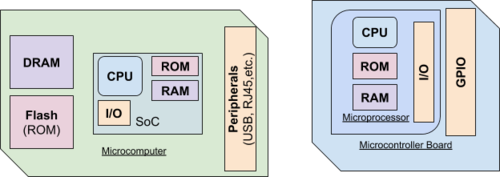
\includegraphics[width=1.0\textwidth]{processor_architectures.png}
    \caption{Microprocessor and microcontroller architectures}
\end{figure}

\subsection{Microcontroller}

Microcontrollers are compact, self-contained computing devices that find use in
embedded systems. They are designed to perform specific tasks with great
efficiency.
A typical microcontroller incorporates a central processing unit (CPU), memory,
input/output pins, and a range of peripherals within a single chip.
This integration minimizes the need for external components, reducing cost,
size, and power consumption.
Microcontrollers excel in real-time control, making them suitable for
applications where precise timing and responsiveness are crucial.
Their versatility, energy efficiency, and cost-effectiveness have made them
the preferred choice in an array of embedded systems, including robotics,
automotive control systems, consumer electronics, and the Internet of Things 
(IoT).

\subsection{Microprocessor}

Microprocessors are the computational brains of modern computing systems.
These general-purpose integrated circuits are designed to process data and
execute instructions efficiently. Unlike microcontrollers, microprocessors
do not integrate a wide array of peripherals, but they offer greater
versatility in terms of the software and hardware components they can work
with.

Microprocessors are commonly found in devices like personal computers,
smartphones, and laptops, where their high processing power is a requirement.
They excel in applications that demand data-intensive tasks, multitasking, and
complex computation.

\subsection{SoC}

System-on-Chip (SoC) integrates multiple components into a single chip, just
like microcontrollers.
The main difference between SoCs and microcontrollers is that the latter can
integrate also GPUs and various acceleraors, making them more complex and
expensive.
The integration of these elements into a single chip enhances efficiency and
reduces power consumption, making SoC really valuable in the embedded systems
world, especially for the automation industy, which could require substantial
processing power for certain applications.

They provide an heterogeneous architecture with different processing units
into the single IC (CPU, GPU, DSP) which can have great performances in
multitask and multithread applications.

\section{Toolchain} 

Developers rely on a set of tools to compile, link, execute and debug software
to a specific target.
Building the firmware images for an embedded system relies on a similar set of
tools, called a toolchain.

In order to create an executable for an embedded system, the process is more
complex than just creating the executable for a regular development
environment.
Since the architecture of the CPU is not the same of the host machine, a
compiler that generates machine code for the specific target architecture is
needed.
The process of creating executable for another architecture is called
cross-compilation and the compiler needs some additional information
to perform it.

\begin{figure}[ht]
    \centering
    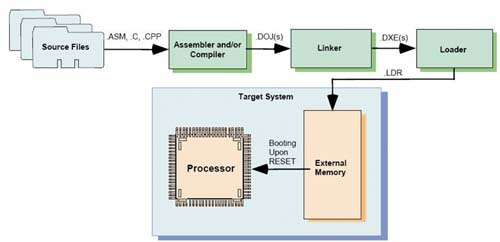
\includegraphics[width=1.0\textwidth]{cross_compilation_process.png}
    \caption{Cross Compilation process}
    \label{fig:cross_compilation}
\end{figure}

\subsection{Cross Compiler}

The first element of the toolchain is the compiler, which is responsible for
translating source code into machine code, which can be interpreted by a
specific CPU.
Each compiler can produce code for only one environment, since the source code
is translated to machine specific instructions, which use the registers and
the address model of a specific architecture.

The compiler creates object files (.o) starting from the source code.
These files contain compiled code for the target machine, which is still not
executable, but can be linked to other object files to create the executable.

Object files contains instructions for the CPU and a symbol table, containing
information about functions and variables of the program.
These files have information about the functions and variables initial value.

\subsection{Linker}

The linker performs the creation of the executable file. It aggregates all the
object files received as input created by the compiler and resolves all the
meaning for every symbol and all the dependencies, finally producing the
executable.

The standard executable format is called ELF (executable and linkable format)
and it has been designed to represent programs on disk and other media.
It can be executed by loading the information in RAM in specific addresses.
ELF files are divided into sections, each one of them represents a different
area of memory with information needed for the execution of the program.
They also contain an header with a pointer to the different sections inside
the file.
The main sections are:

\begin{itemize}
    \item .text: instructions of the program.
    \item .rodata: read only variables.
    \item .data: variables accessible in read and write.
    \item .bss: uninitialized variables which can be accessed in read or write
                mode.
\end{itemize}

Read-only information can be loaded directly from flash in an embedded system,
while data that need to be modified has to be in RAM on modifiable areas of
memory.

In regular development environment, much of the complexity of the linking 
step is hidden, but the linker is configured, by default, to rearrange the
compiled symbols into sections which can be loaded into the process' virtual
addresses by the operating system.

In an embedded system, the linking process becomes more complex as compiled 
symbols have to be placed in physical addresses specific to the system's
architecture.
In order to specify in which areas of memory the sections have to be placed,
a custom linker file has to be created. This file defines the memory layout of
the executable bare metal application.
Additionally, in linker files, custom sections can be used if they are required
by the target system.

\subsection{Make}

GNU Make is a tool which controls the generation of executable and other
non-source files of a program from the program's source files. \cite{GNUMake}
Make gets its knowledge on how to build binary images from a file called
the makefile, which lists how to create each of the non-source files.

The makefile operates on rules and targets. Rules are a series of commands which
instruct make on how to produce a target, representing a non-source file.

One of the advantages of using a build automation tool is that some of the
targets could have implicit dependencies from other intermediate components,
that are automatically resolved at compile time.
It also reduce the time required for the compilation by compiling targets only
when an update to the dependencies has been done.

\subsection{Debugger}

One of the most powerful tools within a toolchain is the debugger. Debuggers
allows developer to test the runtime functionalities of an application,
ensuring it operates as intended or locating the source of errors.

In the host environment, debugging an application consists of launching the
debugger tool with an ELF file as argument or attaching it to a running
application. The standard tool for debugging is called GDB.

However, in embedded development, the situation is slightly different since the
application runs on a different machine than the one used for debugging.
To address this, a version of GDB to debug remote platforms has been developed.
The remote debug session requires an intermediate component which can translate
the GDB commands to CPU specific instructions.

The debug of remote embedded platforms often require a peripheral like JTAG.

\section{Boot}

A bootloader is a piece of software that starts as soon as you power on the
system.
Its primary functionality is to initiate subsequent software components such
as: an operating system, a bare metal application or in some cases another
bootloader.
In the embedded world, bootloaders are intimely tied to the underlying
architecture of the SoC. They are typically securely stored in a non-volatile,
protected on-chip memory, ensuring their availability at startup.

Upon execution, the bootloader executes a series of tasks. It begins by
performing hardware checks to verify the integrity and functionality of the
SoC's components. Then, it takes charge of initializing the processor and
configuring essential system-on-chip registers.

Bootloaders are also important in ensuring security. They often
serve as the starting point for establishing a Hardware Root-of-trust, which
forms the foundation for securing the entire system.

\subsection{Boot steps}

There are several steps that has to be followed for the boot process in an
embedded system.

\begin{figure}
    \centering
    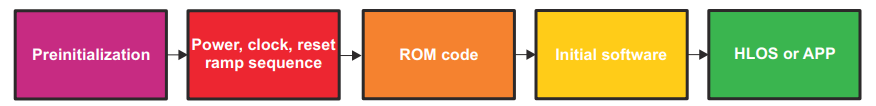
\includegraphics[width=1.0\textwidth]{boot_steps.png}
    \caption{Steps needed for the system boot}
\end{figure}

\begin{enumerate}
    \item   Preinitialization: before the actual boot process begins, certain
            conditions must be met. Power, clock signals, and control
            connections need to be established. Additionaly, boot configuration
            pins should be set to their desired logical levels to configure
            the system's behavior.
    \item   Power, Clock, and Reset Ramp Sequence: the power-management chip
            typically govern the applicaton of a specific sequence for powering
            up the system. This sequence ensures that the system components are
            brought ot life in the correct order and that power and clock
            sources stabilize gradually.
    \item   ROM Code: responsible for finding, for downloading, and for
            executing the initial software (SBL).
    \item   Initial Software (Secondary Bootloader - SBL): software that loads,
            prepares, and passes control to application software or the
            high-level operating system (HLOS).
    \item   High-Level Operating System or Bare-Metal Application: the final
            stage of the boot process involves the execution of the high-level
            operating system or a bare-metal application. This is the primary
            software that runs on the main processor of the system. In case of
            an operating system, it provides a platform for running
            applications. In a bare-metal system, it typically includes the
            main application code that performs specific tasks or functions.
\end{enumerate}

The initial steps of the device initialization process focus on hardware setup,
but they involve configuring system interface pins with software-configurable
functionality. This configuration is an essential part of the chip
configuration and is application dependent.

\subsection{Multi-stage Bootloader}

In advanced SoCs, it is not uncommon for the bootloader to load another
bootloader, creating a multi-stage bootloading process.
In this case the bootloaders serve different purposes.

The initial bootloader, called the first stage bootloader, is typically stored
in a secure, read-only memory for enhanced security and to maintain a
consistent, known state each time the system powers on.
The first stage bootloader is intentionally kept simple and performs only the
essential configuration tasks required to bring up the system.

The secondary bootloader, or second stage bootloader, takes on a more complex
and configurable role to serve the specific needs of the application.
The second stage bootloader can be updated more easily and frequently compared
to the first stage bootloader, making it more adaptable to changes and
enhancements as the system evolves or new features are added.

The multi-stage approach to bootloading exploit the first stage for security
and configuration, while the second one actually initializes the system,
providing modularity and flexibility for future updates.

\begin{figure}[ht]
    \centering
    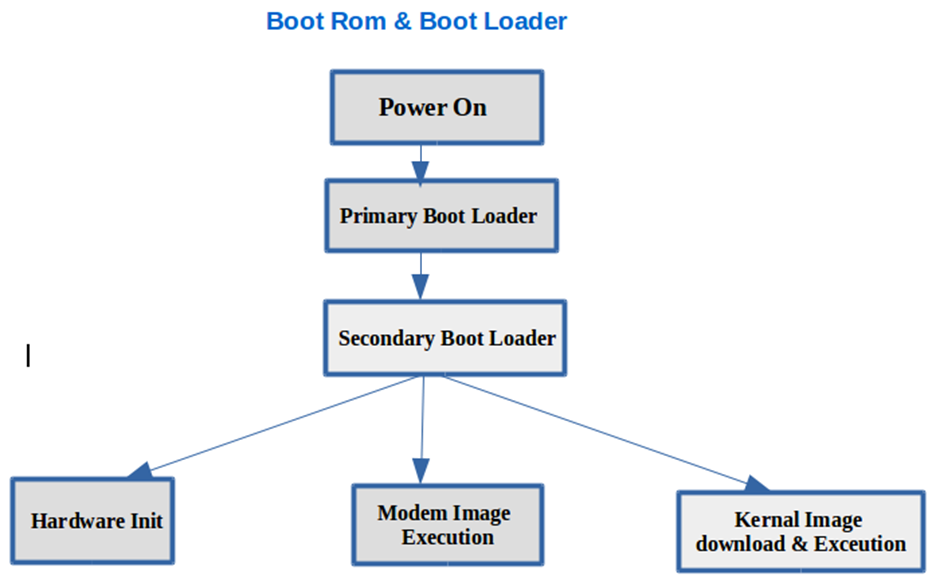
\includegraphics[width=0.7\textwidth]{multi_stage_bootloader.png}
    \caption{Multi stage bootloader}
\end{figure}

\subsection{Multi core bootloading}

Modern embedded systems have multi core architectures that must be initialized,
and the process of bootloading must be carried out by multiple cores, working
together.

Multi core bootloading can be seen as an extension of a multi-stage bootloader.
In this scenario, the first stage bootloader may not even be aware of the
presence of other cores. Its primary responsibility is to initiate the
next-stage bootloader, wihch then takes charge of orchestrating the complex
bootloading process across multiple cores.

The complexities which are introduced in this process are:

\begin{enumerate}
    \item   Image preparation: each processor core may have its own code and
            data segments. The images for each core need to be prepared in a
            specific format that accounts for their individual requirements.

    \item   Image format: the images for every core could be concatenated into
            a single image for the second stage bootloader to load.
            The SBL must be aware of the format used, if only one image is
            used, to correctly parse it.

    \item   Coordination: coordinating the bootloading process across multiple
            cores involves setting up the execution context for each core,
            initializing hardware components, and synchronizing the start of
            execution. The SBL takes on the role of managing these tasks to
            ensure a smooth and reliable multi-core startup.
\end{enumerate}

\section{Operating Systems}

In the embedded world there are different kind of operating systems, not only
realized by different companies, but also with different needs as objective.
Embedded devices, usually, needs to satisfy real time requirements, which
makes hard using a general operating system, since they can not provide
this feature.

The essence of real time is not that a computer has to respond fast, but that
it has to respond reliably fast.
The requirement of real time programming is being able to quickly handle
aynchronous events. \cite{abbott2011linux} 

For many years, the only solution used for these devices was the bare metal
approach. In this case there is not a real operating system which takes care
of the management of fundamental operations.
A bare metal application is considered to run directly on the hardware without
respecting an external programming interface 
(e.g., the one given by an operating system), having direct access to CPU
or microcontroller registers and without the security mechanisms of an OS.

Bare metal programming has the advantage of providing to the developers the
highest grade of freedom, understanding exactly what every action will end up
doing. Bare metal applications has the greatest possible degree of 
determinism and the resouce consumption is optimized for the specific case. 
On the other hand, it becomes hard to manage large project with different tasks
and multiple operations to perform.

Other than the bare metal approach, there is the possibily of running a Real
Time Operating System, which provides support for multiple tasks and
device drivers between the hardware and the application, stack for the network
and security.

\subsection{Real Time Operating Systems}

As the complexity of tasks continue to increase for embedded devices the
necessity for a RTOS has increased and always more embedded devices go towards
this solution, leaving behind the bare metal approach.
These systems gives an efficient solution to meet hard real time requirements,
particularly in safety critical applications that requires the management of
different safety applications on the same device.

The scheduler in a RTOS, which has the job of deciding which thread have to
execute on the core in any moment, is made in such a way to guarantee 
deterministic execution pattern. Real Time schedulers achieve determinism by
assigning a priority to each task. In this way the scheduler can always run the
task with the highest priority. \cite{freeRTOS}

\subsubsection{FreeRTOS}

FreeRTOS is a real-time operating system kernel for embedded devices. It is
designed to be small and simple, built with an emphasis on reliability and
ease of use.
It is ideally suited for real-time applications, including a mix of both
soft and hard real time requirements.

FreeRTOS allows applications to be organized as a collection of independent
threads of execution. On a single core processor, only one thread can execute
in any given time. The kernel decides which thread should be executing by
examining the priority assigned to each threda by the application designer.
Typically, threads with hard real-time requirements have higher priorities,
ensuring their execution ahead of threads with soft real-time requirements.

In a single core system, the CPU must divide the tasks into time slices so that
they can appear to run concurrently. The scheduler in an operating system is
charged with figuring out which task to run each time slice.
In FreeRTOS, the default time slice is 1 millisecond, referred to as "tick". 
A hardware timer is configured to create an interrupt every 1 ms and
the handler for that interrupt runs the scheduler, which chooses the task to
run next.
At eahch tick interrupt, the task with the highest priority is chosen to run.
If the highest priority tasks have the same priority, they are executed in a
round-robin fashion. If a task with an higher priority than the currently
running task becomes available, then it will immediately run, withoug waiting 
for the next tick.

\begin{figure}[htb]
    \centering
    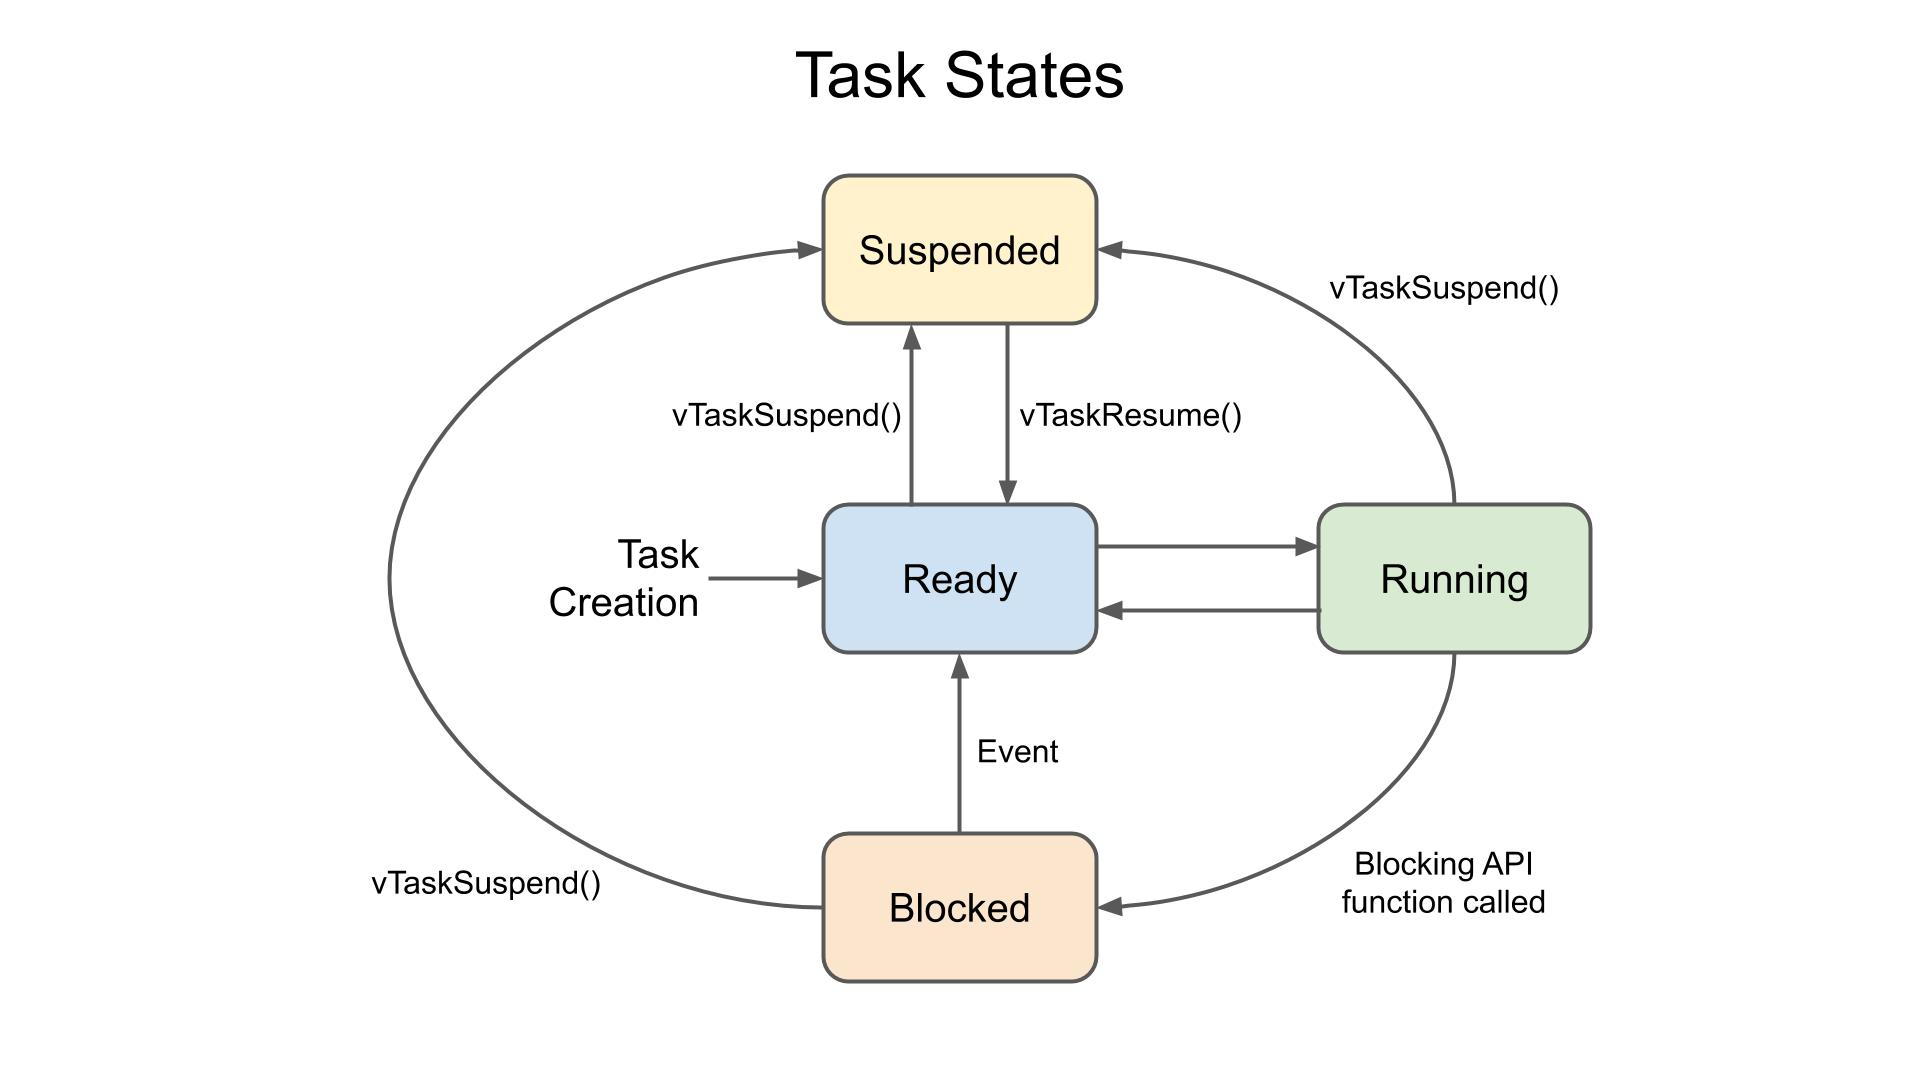
\includegraphics[width=1.0\textwidth]{task_states.jpeg}
    \caption{Task states}
\end{figure}

As soon as a task is created, it enters the Ready state, signaling their
readiness to the scheduler for potential execution.

In multi core systems, the scheduler can schedule tasks based on the number of
available cores in the system.

In addition, FreeRTOS provides features to simplify the embedded software
development. It includes services for task scheduling, synchronization
primitives, resource management, and interrupt handling.

\subsection{Linux Embedded Systems}

Embedded Linux is built on the same Linux kernel of every other linux systems.
Other than the Linux kernel, embedded applications need additional packages,
which depends on the distribution and can be chosen based on the necessities
of the developer. ~\cite{embedded_linux_windriver}

\begin{figure}
    \centering
    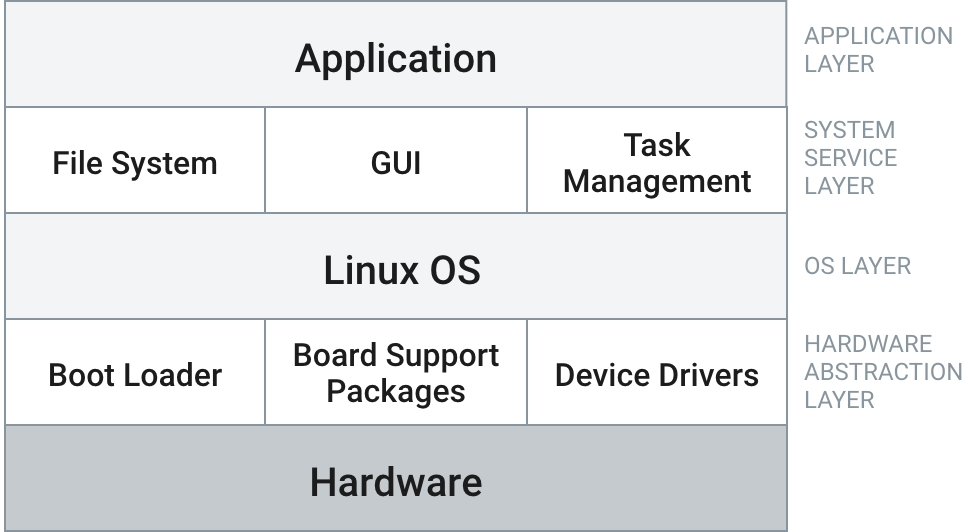
\includegraphics[width=1.0\textwidth]{embedded_linux_architecture.jpg}
    \caption{Embedded Linux Architecture}
    \label{fig:embedded_linux_architecture}
\end{figure}

Although most of the devices are small in size, there are some of them that can
run a version of the GNU/Linux operating system. To have this possibility the
device must of a reasonable amount of RAM and the hardware must support MMU,
Memory Management Unit, to provide different virtual address spaces for every
process.

The main advantage of using a system with Linux is that the opportunity for a
tailored soluion will be less, since the requirements, resource wise, for
running Linux makes a system overkill for most of the applications.
In this way, the software design can be simpler and it is possible to use
existing solutions to embedded problems.

On the other hand, embedded devices have in many cases hard real time
requirements, meaning that a series of operations must be accomplished in a
short, measurable, predictable amount of time. To accomplish this Real-Time
Operating Systems are used and it is almost impossible to achieve real time
processing with embedded Linux as operating system, even if some patches 
to the kernel's scheduler have been applied to help meet these requirements.

Other application domains for embedded devices are low power consumptions,
which could run on a battery or energy harvesting device. In this case, having
an operating system increase the energy need of the device.

A reason for which linux could be a perfect candidate as an operating system
for embedded devices is its modularity. Embedded developers have the
possibility to customize their linux distribution, including only the necessary
parts for their use case. \cite{linux_embedded_ubuntu}

\subsubsection{Linux Embedded Real Time}

One way to improve real time performances in an operating system is to add
extra preemption points, where the OS can switch to critical operations.
However, this process worsen the overall performances of the operating system
in the general case, which is what general systems are optimized for, not
taking into consideration the worst-case scenario, making the system
non-deterministic. 

The solution to the problem is to decouple the real time part of the system
from the general purpose kernel.
It is possible to optimize the real time OS to meet deadlines, having the best
performance of general computing. \cite{linux_real_time} 

Different projects to integrate real time into linux have been realized
(e.g., RTLinux, RTAI).
Although, they are maintained by different people, most of the functionalities
are the same between different projects:

\begin{itemize}
    \item A small real time core.
    \item One shot and periodic timer support.
    \item Real time scheduler.
    \item Real time threads.
    \item Real time FIFOs and shared memory.
    \item Real time interrupt handler.
\end{itemize}

\begin{figure}[htb]
    \centering
    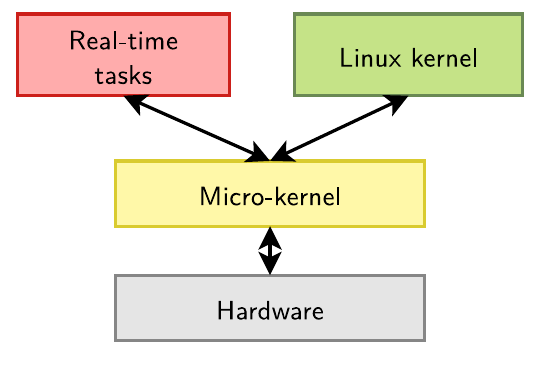
\includegraphics[width=1.0\textwidth]{real_time_linux_architecture.png}
    \caption{Architecture of Real Time Linux}
    \label{fig:real_time_linux_architecture}
\end{figure}

\subsubsection{Yocto}

The Yocto Project is an open source project that helps developer create a
custom Linux based systems independently from the hardware architecture.
\cite{yocto}
Yocto is used to create operating system containing only the features
needed by the embedded application. 
The Yocto project is more than a build system. It provides tools, processes,
templates and methods so developers can rapidly create and deploy products for
the embedded market.

\begin{figure}[htb]
    \centering
    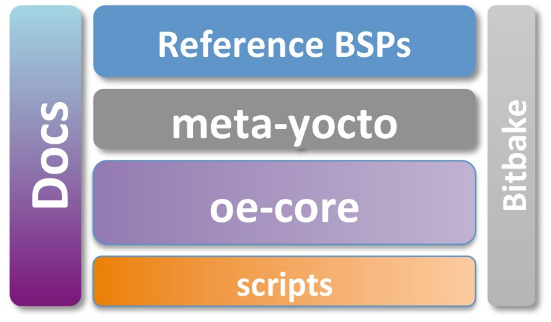
\includegraphics[width=1.0\textwidth]{yocto_stack.png}
    \caption{Yocto Stack}
    \label{fig:yocto_stack}
\end{figure}

Yocto makes possible to automize the creation of an embedded operating system.
The needed steps to develop a system are:

\begin{enumerate}
    \item   Select and download the necessary packages and components.
    \item   Configure the downloaded packages.
    \item   Compile the configured packages.
    \item   Install the generated binary, libraries, etc.
    \item   Generate the final deployable format.
\end{enumerate}

Depending on the number of packages needed, these steps could become really
complex to manage, making preferable to use an automated system.

Yocto is characterized by a layer model which grants modularity and the
possibility for different developers to work on different part of the system
at the same time.

Layers are a set of instructions that tells the build system what to do
and they are used to logically separate information in a specific build.

Yocto is formed by two main components: bitbake and OE-Core (Open Embedded core).
They are combined to realize the poky host build.

The OpenEmbedded-Core is a collection of information, such as configuration
files and recipes used as a common layer to create the custom distributions.
It is the starting point from which every distribution is built.

Bitbake is a build engine, which analyze files called recipes, and build an
image from them. Inside the recipes there will be all the instruction the
engine has to perform to create the image.

The project's strenght lies in its ability to offer customization,
cross-compilation support, reporducibiliy and a community ecosystem, making it
a fundamental tool for crafting optimized Linux-based solutions for embedded
applications.

\subsubsection{Poky}

Poky is the Yocto project reference distribution and is composed of a
collection of tools and metadata.
It contains the OpenEmbedded Build system: BitBake and OpenEmbedded Core.
It also include a large set of recipes, organized in hierarchical layers.
It provices the mechanism to build and combine thousands of distributed open
source projects to form a fully customizable, complete and coherent Linux
software stack. \cite{salvador2014embedded}

\begin{figure}[ht]
    \centering
    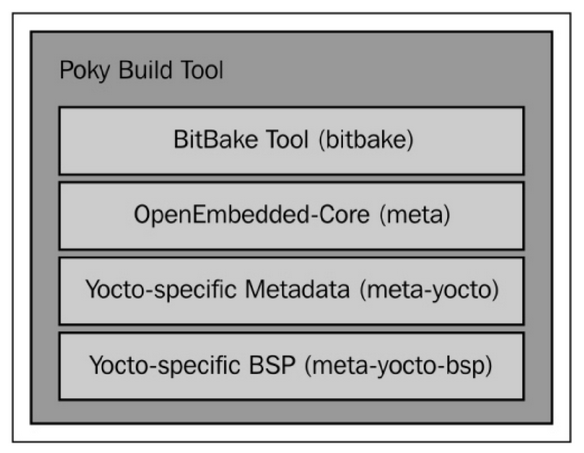
\includegraphics[width=1.0\textwidth]{yocto_poky_stack.png}
    \caption{Poky build tool stack}
\end{figure}

The main concept on which the Poky Build System is constructed is that every
aspect of a build is controlled by metadata, grouped into package recipes.
A recipe is then used by BitBake to set variables or define additional tasks to
be performed during the build.
